\begin{answer}

    \begin{minipage}{0.48\textwidth}
        \centering
        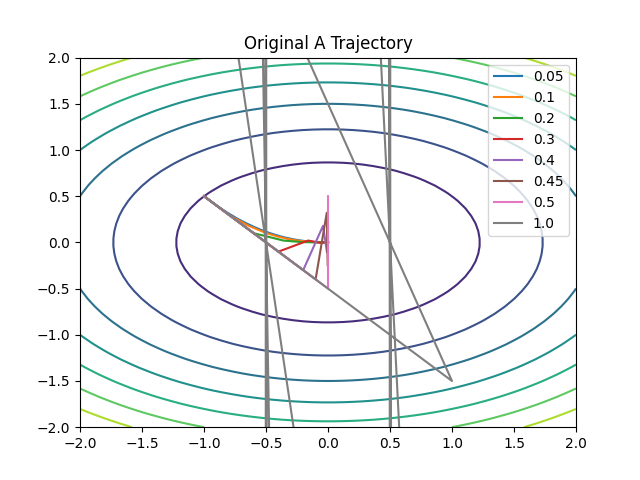
\includegraphics[width=\textwidth]{src/gd_convergence/trajectories.png}
        \captionof{figure}{Gradient descent trajectories \\ with regular A.}
        \label{fig:gd-trajectories}
    \end{minipage}
    \hfill
    \begin{minipage}{0.48\textwidth}
        \centering
        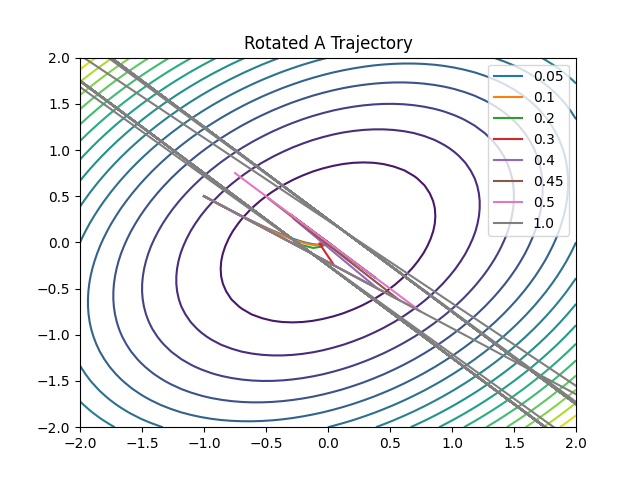
\includegraphics[width=\textwidth]{src/gd_convergence/trajectories_rotated.png}
        \captionof{figure}{Gradient descent trajectories \\ with rotated A.}
        \label{fig:gd-trajectories-rotated}
    \end{minipage}

    \vspace{1em}    

   As predicted by our result in a2), we can see that with very small learning rates GD takes a lot of steps to converge, same as with larger learning rates after a specific point (~ $\alpha$ > 0.3), as they tend to overshoot. After $\alpha$ > 0.5 GD doesn't seem to converge anymore and either the loss stays constant or increases until we stop after hitting our thresholds

\end{answer}